\documentclass[margin=10pt]{standalone}
\usepackage[utf8]{inputenc}
\usepackage{tikz}
\usetikzlibrary{
    shapes, 
    arrows, 
}
%
\newcommand{\xfeature}{$x_1$}
\newcommand{\yfeature}{$x_2$}
\newcommand{\nodewidth}{1em}
\newcommand{\nodeheight}{1em}
\newcommand{\nodedistance}{3em}
\newcommand{\leveldistance}{5em}
%
\tikzstyle{treearrow} = [->,-To, shorten >=1pt]
%
\tikzstyle{treenode} = [
  draw,     
  shape=rectangle,
  color=black,
  solid, 
  minimum width=\nodewidth,
  minimum height=\nodeheight,
]
%
\tikzstyle{rareclass} = [
  draw,
  shape=rounded rectangle,
  color=black,
  fill=yellow,
  solid, 
  minimum width=\nodewidth,
  minimum height=\nodeheight,
]
%
\tikzstyle{nonrareclass} = [
  draw,     
  shape=rounded rectangle,
  color=black,
  solid, 
  minimum width=\nodewidth,
  minimum height=\nodeheight,
]
%
\begin{document}
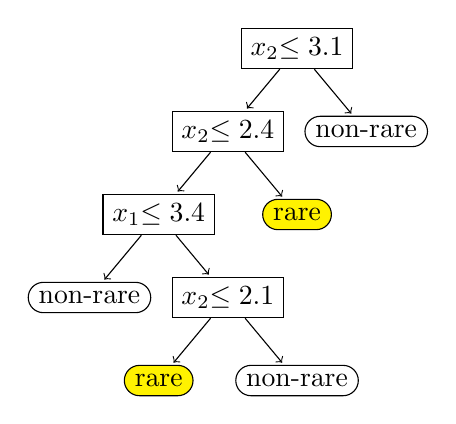
\begin{tikzpicture}[
    level distance=\nodedistance,
	level 1/.style={sibling distance=\leveldistance},
	level 2/.style={sibling distance=\leveldistance},
    every node/.style={transform shape},
    ]
    \node[treenode, anchor=north] (dtree) at (10, 0) {\yfeature $\le 3.1$}
    child { node[treenode] {\yfeature $\le 2.4$} edge from parent [treearrow]
      child { node[treenode] {\xfeature $\le 3.4$}
      child { node[nonrareclass] {non-rare} }
      child { node[treenode] {\yfeature $\le 2.1$}
          child { node[rareclass] {rare} }
          child { node[nonrareclass] {non-rare} } 
        }
      }
      child { node[rareclass] {rare} }
    }
    child { node[nonrareclass] {non-rare} edge from parent [treearrow] };
\end{tikzpicture}
\end{document}